% -*- latex -*-
%%%%%%%%%%%%%%%%%%%%%%%%%%%%%%%%%%%%%%%%%%%%%%%%%%%%%%%%%%%%%%%%
%%%%%%%%%%%%%%%%%%%%%%%%%%%%%%%%%%%%%%%%%%%%%%%%%%%%%%%%%%%%%%%%
%%%%
%%%% This text file is part of the theory writeup on the
%%%% Integrative Model for Parallelism,
%%%% copyright Victor Eijkhout (eijkhout@tacc.utexas.edu) 2014-6
%%%%
%%%% shortthreepoint.tex : include file for IMP-11
%%%%
%%%%%%%%%%%%%%%%%%%%%%%%%%%%%%%%%%%%%%%%%%%%%%%%%%%%%%%%%%%%%%%%
%%%%%%%%%%%%%%%%%%%%%%%%%%%%%%%%%%%%%%%%%%%%%%%%%%%%%%%%%%%%%%%%
\Level 1 {Threepoint averaging example}

For a realistic example, we create a sequence of objects and a sequence of kernels
that are all added to the algorithm:
\begin{verbatim}
IMP_object **all_objects = new IMP_object*[nsteps+1];
for (int step=0; step<=nsteps; ++step) {
  IMP_object
    *output_vector = new IMP_object( blocked );
  all_objects[step] = output_vector;
  IMP_object
    *input_vector = all_objects[step-1],
    *input_vector = all_objects[step];
  IMP_kernel *update_step = 
    new IMP_kernel(input_vector,output_vector);
  // other steps for the kernel are as above
}
\end{verbatim}
After that we call
\begin{verbatim}
algorithm->analyze_dependencies();
algorithm->execute();
\end{verbatim}
as before.

\subsection {Comparison to reference code}

OpenMP: We compared the threepoint averaging kernel on $3\times 10^7$
elements, running on one node of the Stampede supercomputer at the
Texas Advanced Computing Center
(\url{http://www.tacc.utexas.edu/stampede}). The IMP implementation
and the OpenMP reference both use the
OpenMP~v3 task mechanism. Figure~\ref{fig:omp-scale} 
then shows that the overhead of the IMP mechanisms is negligible.
\begin{figure}[ht]
  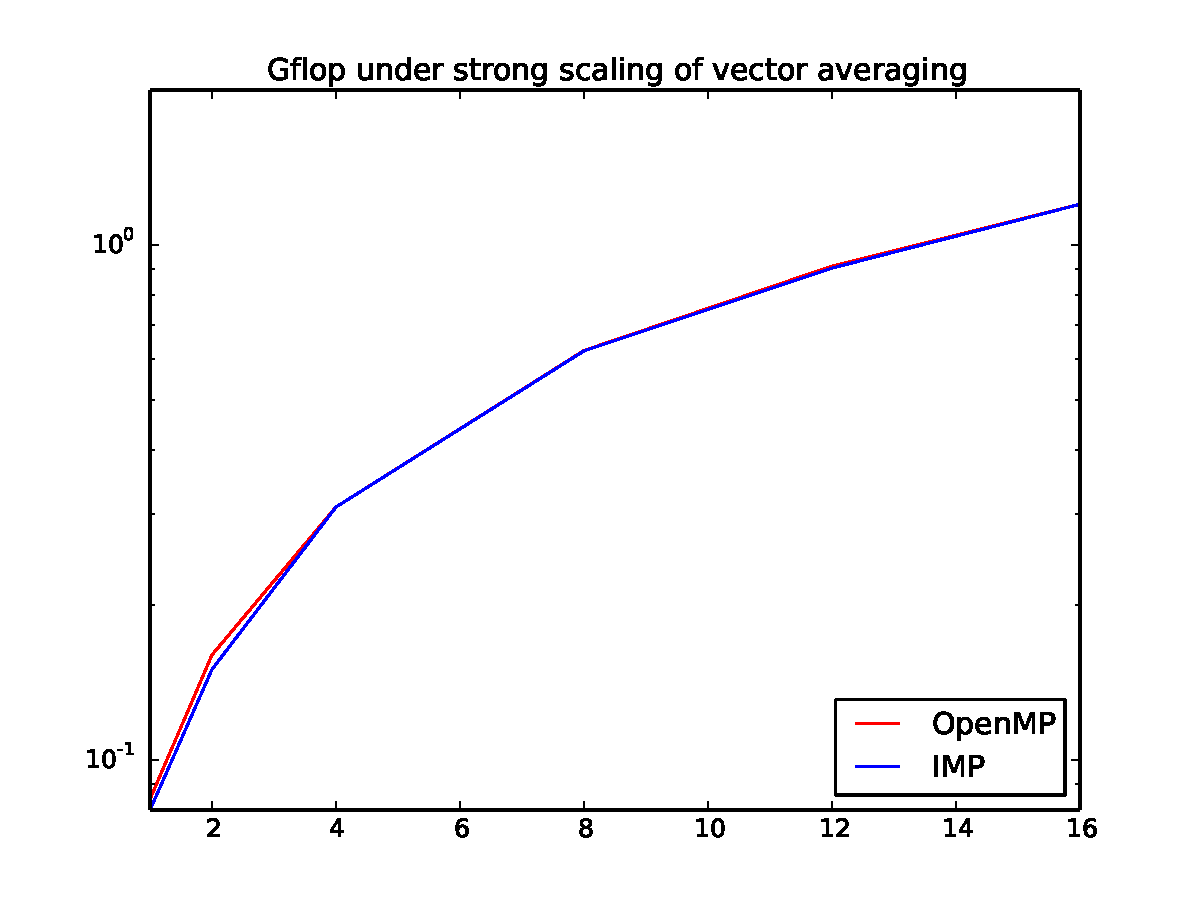
\includegraphics[scale=.4]{omp_scaling}
  \caption{Strong scaling of IMP/OMP code versus OpenMP reference code
    as a function of core count}
  \label{fig:omp-scale}
\end{figure}
Both tasking codes do not show approximately linear scaling, probably
because of the excess of available bandwidth at low core/thread
counts.

MPI: We wrote an MPI code that performs the left/right sends
hardwired. Since the IMP code is general in its treatment of 
communication patterns, it includes a preprocessing stage that is absent
from the `reference' code. We did not include it in the timings since
\begin{enumerate}
\item Preprocessing will in practice be amortized, and
\item For irregular problems an MPI code will have to perform a 
  very similar analysis, so the choice of our test problem made the reference
  code unrealistically simple.
\end{enumerate}
\begin{figure}[ht]
  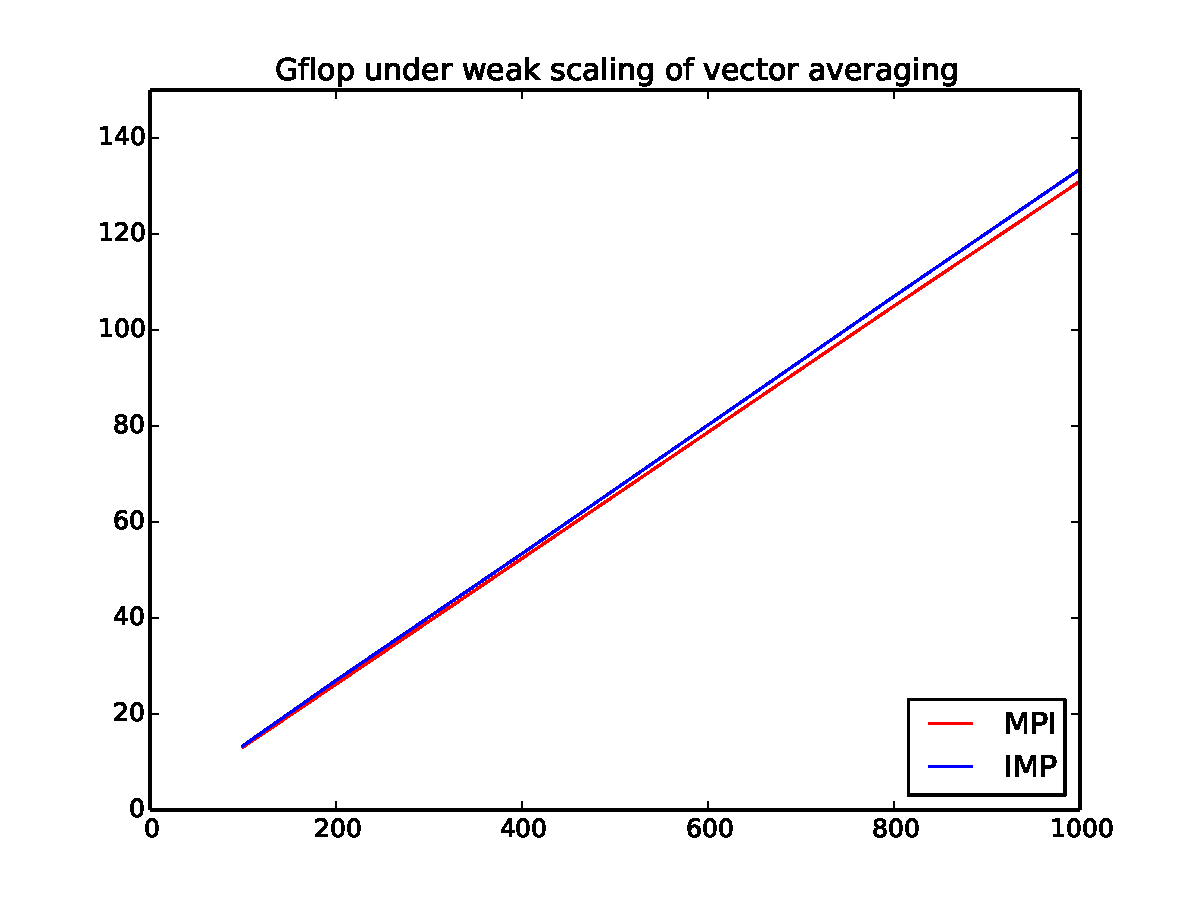
\includegraphics[scale=.4]{mpi_scaling}
  \caption{Weak scaling of IMP/MPI code versus MPI reference code
    as a function of core count}
  \label{fig:mpi-scale}
\end{figure}
Figure~\ref{fig:mpi-scale} shows the behaviour.  Since the two codes
do essentially the same thing it is not surprising to see the same
perfect linear scaling from both. (It is not clear why the IMP code is
in fact 2--3\% faster.)

\begin{comment}
  \heading{Discussion of the prototype}

  We address a few possible criticisms of the prototype.
  \begin{description}
  \item[Limitations] This example uses a 1D distribution, but 2D and sparse
    distributions are possible.
  \item[Regarding the originality of distributions] The concept of
    distribution is not new. However, the innovation here lies in the
    fact that distributions are also used as a tool for describing the
    algorithm. Thus, the IMP translator can relate data storage and
    data requirements, and thus come up with an efficient
    implementation.
  \item[Synchronous vs asynchronous] The IMP kernels seem to imply a notion of
    BSP-like supersteps. This is not the case: the kernels translate to a dataflow
    \ac{IR} which can be executed fully asynchronously.
  \item[Function pointer callbacks] The above implementation of the 1D
    example uses callbacks. These would not be necessary in an MPI
    realization, but they \emph{are} necessary for a task-based
    interpretation. For MPI, the system allows you to execute a kernel
    directly.
  \end{description}
\end{comment}

\subsection{Further discussion}

We argued above that the key to the success of \ac{IMP}
is the fact that the $\beta$-distribution
is explicitly known. This can be achieved through various
mechanisms for defining the indirect function~$I_f$..
We have the following options.
\begin{itemize}
\item The example above derived the $\beta$-distribution through applying
  operators on the $\alpha$-distribution.
\item The $\alpha\rightarrow\beta$ mapping is conceptually a boolean sparse matrix.
  For sparse problems such as from \acp{PDE} this is indeed how we specify it:
\begin{verbatim}
void set_index_pattern( index_pattern *patt );
\end{verbatim}
\item For kernels that are a strictly local operation that needs to be declared:
\begin{verbatim}
void set_type_local();
\end{verbatim}
\item For collectives, one can show that $\beta=\gamma$, so this is specified as
%% imp_distribution 
%%     *localscalar = new imp_distribution(env,"disjoint-block",1,-1),
%%     *gathered_scalar = new imp_gathered_scalar(env);
%% imp_object
%%     *localvalue = new imp_object(localscalar),
%%     *gatheredvalue = new imp_object(gathered_scalar);
\begin{verbatim}
imp_kernel
    *gather = new imp_kernel(localvalue,gatheredvalue);
gather->set_explicit_beta_distribution(gathered_scalar);
\end{verbatim}
\item Finally, we can also specify it by giving the $I_f$ function explicitly:
\begin{verbatim}
void set_indirect_function( indexstruct*(*f)(index_int) );
\end{verbatim}
\end{itemize}
